\chapter{Theory: Frequency Dependent Squeezing \& Membrane based Optomechanics}
This chapter will cover the elementary concepts required to describe an membrane based optomechanical system in a quantum regime. We will first recall basics on optical field quantization as well describing coherent and squeezed light field, to then turn to the more specific frequency dependent squeezed light field. Secondly, we will cover the mathematical description of a mechanical resonator interacting with a generic coherent optical field, highlighting the differences with the seminal optomechanical system of a mirror on a spring. Finally, we will derive the equations of motions of a membrane based optomechanical system with frequency dependent squeezed optical fields. 
\newpage
\minitoc
\newpage


\section{Squeezed Light and Optomechanics}

We will now introduce the concept of Standard Quantum Limit (SQL) in the context of optomechanical measurements, and show how frequency dependent squeezed light can be used to surpass this limit. \\ 

For the rest of this section we will assume the following
\begin{itemize}
  \item A cavity on resonance: $\Delta=0$.
  \item A single port optomechanical cavity: $\kappa_1 \sim \kappa$ .
  \item The unresolved sideband regime: $(\Omega, \Omega_m) \ll \kappa/2$.
\end{itemize}
\subsection{Standard Quantum Limit}
The question of interest is now:
\begin{center}
  \textbf{what is the best displacement sensitivity one can achieve?}
\end{center}  

We start by recalling the reflected phase fluctuation of an optomechanical cavity from section II.2.5 under the aforementioned assumptions:
\begin{equation*}
\delta \hat{q}_r[\Omega] = \, \delta \hat{q}_{\mathrm{in}}[\Omega]  + \mathcal{K}[\Omega]\, \delta \hat{p}_{\mathrm{in}}[\Omega] \quad  \text{with} \quad \mathcal{K}[\Omega] =  \dfrac{128 \hbar \mathcal{F}^2 \bar I_{\rm in}}{\lambda^2}  \,  \chi[\Omega]
\end{equation*}
as well as the phase to displacement transduction relation with an optomechanical escape efficiency of 1:
\begin{equation*}
   \delta \hat q_x = \frac{16 \mathcal{F}\sqrt{\bar I_{\rm in}}}{\lambda}\delta \hat{x}[\Omega]  
\end{equation*}
Using these two relations, we can then express displacement fluctuations in terms of input amplitude and phase fluctuations, assuming the reflected field is a perfect probe of the mechanical resonator position fluctuations i.e. $\delta \hat q_r[\Omega] = \delta \hat q_x[\Omega]$. This treatment is formally equivalent to considering the output phase as a statistical estimator of the position fluctuations being a stationary random process as done in quantum measurement theory \cite{clerk_introduction_2010}. We then write
\begin{equation}
  \delta \hat{x}[\Omega] = \frac{\lambda }{16 \mathcal{F}\sqrt{\bar I_{\rm in}}} \, \delta \hat{q}_{\mathrm{in}}[\Omega]  + \dfrac{8 \hbar \mathcal{F}\sqrt{\bar I_{\rm in}}}{\lambda} \, \chi[\Omega] \, \delta \hat{p}_{\mathrm{in}}[\Omega]
\end{equation}
such that the associated displacement spectrum reads
\begin{equation}
      S_{xx}[\Omega] = \dfrac{\lambda^2}{256 \mathcal{F}^2 \bar{I}_\mathrm{in}} S_{qq}^{\rm in}[\Omega] +  \dfrac{64 \hbar^2 \mathcal{F}^2 \bar{I}_\mathrm{in}}{\lambda^2}|\chi[\Omega]|^2 S_{pp}^{\rm in}[\Omega]  \quad  + \hbar |\chi[\Omega]| \Re\Big[  e^{i\phi_m[\Omega]} S_{pq}^{\rm in}[\Omega]\Big]
  \label{eq:total_displacement_spectrum}
\end{equation}

We then identify three contributions to the displacement spectrum:
\begin{itemize}
  \item The first term is the laser shot noise (or imprecision noise) scaling inversely with the input power $\bar{I}_\mathrm{in}$, arising from the input phase fluctuations $S_{qq}^{\rm in}[\Omega]$ and given by
  \begin{equation}
    S_{xx}^{\rm SN}[\Omega] = \dfrac{\lambda^2}{256 \mathcal{F}^2 \bar{I}_\mathrm{in}} S_{qq}^{\rm in}[\Omega]
  \end{equation}
  \item The second term is the radiation pressure noise (or backaction noise) scaling linearly with the input power $\bar{I}_\mathrm{in}$, arising from the input amplitude fluctuations $S_{pp}^{\rm in}[\Omega]$ driving the mechanical resonator via radiation pressure given by 
  \begin{equation}
    S_{xx}^{\rm RPN}[\Omega] = \, \dfrac{64 \hbar^2 \mathcal{F}^2 \bar{I}_\mathrm{in}}{\lambda^2}|\chi[\Omega]|^2 S_{pp}^{\rm in}[\Omega]
  \end{equation}
  \item The third term is a correlation term between amplitude and phase fluctuations $S_{pq}^{\rm in}[\Omega]$, which can be non-zero for arbitrary squeezed states as seen in the previous section and given by
  \begin{equation}
    S_{xx}^{\rm cor}[\Omega] = \hbar |\chi[\Omega]|\Re\Big[ e^{i\phi_m[\Omega]} S_{pq}^{\rm in}[\Omega]\Big]
  \end{equation}
\end{itemize}
And we write the total displacement spectrum as the sum of these three contributions
\begin{equation}
  S_{xx}[\Omega] = S_{xx}^{\rm SN}[\Omega] + S_{xx}^{\rm RPN}[\Omega] + S_{xx}^{\rm cor}[\Omega]
\end{equation}

We now consider vacuum/coherent fluctuations such that $S_{qq}^{\rm in}[\Omega]=S_{pp}^{\rm in}[\Omega]=1$ and $S_{pq}^{\rm in}[\Omega]=0$, so that the displacement spectrum simplifies to
\begin{equation}
  S_{xx}[\Omega] = \dfrac{\lambda^2}{256 \mathcal{F}^2 \bar{I}_\mathrm{in}} +  \dfrac{64 \hbar^2 \mathcal{F}^2 \bar{I}_\mathrm{in}}{\lambda^2}|\chi[\Omega]|^2 
  \label{eq:total_displacement_spectrum}
\end{equation}
and we look at what noise dominates the displacement spectrum around the mechanical resonance $\Omega \sim \Omega_m$. We define the frequency $\Omega_{\text{SQL}}$ as the frequency at which the SQL is achieved, given by
\begin{equation}
  \Omega^{\pm}_{\text{SQL}}  =\;\sqrt{\Omega_m^2-\dfrac{\Gamma_m^2}{2}
\;\pm\;\dfrac{1}{2}\sqrt{\Gamma_m^4-4\Gamma_m^2\Omega_m^2+\Big(\frac{256\,\hbar\,\mathcal F^2 I_{\rm in}}{m\lambda^2}\Big)^2}}
\end{equation}
and consistent with the LIGO/Virgo notation \cite{harry_advanced_2010, aasi_enhanced_2013}. Over the frequency range of interest $\Omega \in [\Omega_m - \Omega_{\text{SQL}}, \Omega_m + \Omega_{\text{SQL}}]$, the displacement noise is dominated by the radiation pressure noise, while outside this range, the noise is dominated by the shot noise. However, for every sideband frequency, there exists an optimal input power $\bar{I}_\mathrm{in}^{\rm SQL}[\Omega]$ at which both contributions are equal, minimizing the total displacement noise. This limit is called the Standard Quantum Limit (SQL) and is a direct consequence of Heisenberg's uncertainty principle applied to continuous position measurements \cite{braginsky_quantum_1992, clerk_introduction_2010}. This SQL intensity is given by
\begin{equation}
  S_{xx}^{\rm SN}[\Omega] = S_{xx}^{\rm RPN}[\Omega] \implies \bar{I}_\mathrm{in}^{\rm SQL}[\Omega] = \dfrac{\lambda^2}{128\mathcal{F}^2 \hbar |\chi[\Omega]|}
\end{equation}
such that plugging back in this SQL intensity in \eqref{eq:total_displacement_spectrum} gives the SQL displacement spectrum as
\begin{equation}
  S_{xx}^{\rm SQL}[\Omega] = \hbar |\chi[\Omega]| \implies S_{xx}^{\rm SN}[\Omega] + S_{xx}^{\rm RPN}[\Omega] \geq \hbar |\chi[\Omega]|
\end{equation}
which is the fundamental limit to continuous position measurements with coherent light. We also note that for high Q resonators, $\Omega_{SQL} \ll \Gamma_m$, so approximating the succeptibility by its real part holds over a relatively large frequency range.

\subsubsection{Thermal Noise}
Thermal noise is a major limitation in optomechanical experiments, as it can mask the quantum effects one aims to observe. The mechanical resonator is indeed coupled to a thermal bath at temperature $T$, which drives the resonator into a thermal state with mean phonon occupation number $\bar n_{\mathrm{th}} = k_B T / (\hbar \Omega_m)$ in the high temperature limit $k_B T \gg \hbar \Omega_m$. The position fluctuations induced by this thermal force is given by
\begin{equation}
  S_{xx}^{\mathrm{th}}[\Omega] = \dfrac{2\hbar}{1 - e^{-\hbar \Omega / k_B T}} \Im \chi[\Omega] \simeq 2 m \Gamma_m k_B T |\chi[\Omega]|^2 \quad \text{if} \quad k_B T \gg \hbar \Omega
\end{equation}
where we used the identity $\Im \chi[\Omega] = m\Gamma_m \Omega |\chi[\Omega]|^2$. At $T=0K$, this reduces to the zero point fluctuations spectrum $S_{xx}^{\mathrm{ZPF}}[\Omega] =\, m \Gamma_m \hbar \Omega_m  |\chi[\Omega]|^2 < $$S_{xx}^{\rm SQL}[\Omega]$, such that is often neglected in the total displacement spectrum. However, at finite temperature, the thermal noise can be much larger than the SQL. Therefore, the total displacement spectrum now reads
\begin{equation}
  S_{xx}[\Omega] = S_{xx}^{\rm SN}[\Omega] + S_{xx}^{\rm RPN}[\Omega] + S_{xx}^{\rm cor}[\Omega] + S_{xx}^{\mathrm{th}}[\Omega]
\end{equation}
In order to experimentally probe these quantum limits without being limited by various technical noises, one would then need: 
\begin{itemize}
  \item A high finesse cavity, such that the shot noise $S_{xx}^{\rm SN} \propto \mathcal{F}^{-2}$ level is low, and the radiation pressure noise $S_{xx}^{\rm RPN} \propto \mathcal{F}^{2}$ is high. One should however ensure the cavity bandwidth $\kappa$ is still much larger than the mechanical frequency $\Omega_m$. This can be ensure tuning the cavity length $L$ and mirror transmissions.
  \item A low mass, low frequency, high quality factor mechanical resonator, such that the susceptibility modulus at resonance $|\chi[\Omega_m]|=Q/m \Omega_{m}^2$ is high, and it comes out of the shot noise level significantly. 
  \item A low temperature environment, such that the thermal noise $S_{xx}^{\mathrm{th}} \propto T$ is low and does not mask the quantum effects. This can be ensured by cryogenic cooling of the mechanical resonator, as well as using high quality factor resonators to reduce the mechanical linewidth $\Gamma_m$.
\end{itemize}

\begin{figure}
  \centering
  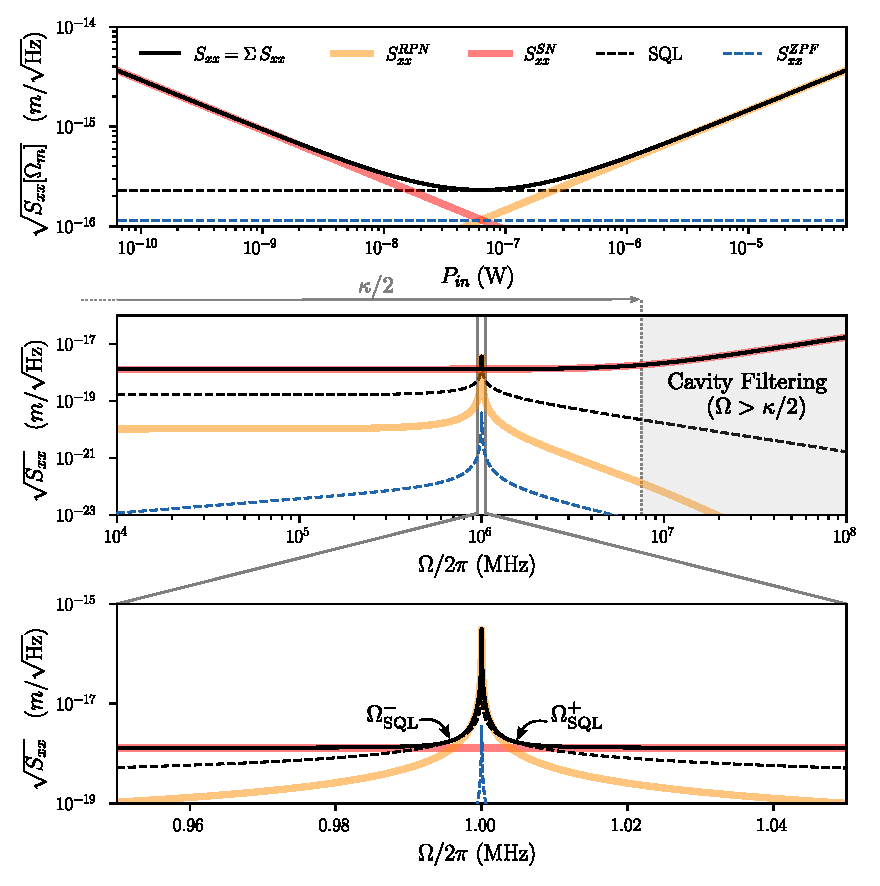
\includegraphics[width=\textwidth]{./chap3/fig/SQL0.pdf}
  \caption{DYes}
  \label{fig:freq_indep_squeezing}
\end{figure}

We now want to derive the displacement spectrum of an optomechanical system driven by a squeezed light field, whether frequency independent or dependent. 

\subsection{Frequency Independent Squeezing in Optomechanical Cavities}
We first recall the (idealized) covariance matrices for both a phase squeezed field and an amplitude squeezed field 
\begin{equation*}
  \mathbf{S}^{0}_{\rm OPO}[\Omega] = 
  \begin{pmatrix}
    e^{+2r} & 0\\
    0 & e^{-2r}
  \end{pmatrix}, \quad
  \mathbf{S}^{\pi}_{\rm OPO}[\Omega] = 
  \begin{pmatrix}
    e^{-2r} & 0\\
    0 & e^{+2r}
  \end{pmatrix}
\end{equation*}
For a phase squeezed field, the displacement spectrum reads
\begin{equation}
  S_{xx}^{0}[\Omega] = \dfrac{\lambda^2}{256 \mathcal{F}^2 \bar{I}_\mathrm{in}}  e^{-2r} + \dfrac{64 \hbar^2 \mathcal{F}^2 \bar{I}_\mathrm{in}}{\lambda^2}|\chi[\Omega]|^2 e^{+2r}
\end{equation}
while for an amplitude squeezed field, the displacement spectrum reads
\begin{equation}
  S_{xx}^{\pi}[\Omega] = \dfrac{\lambda^2}{256 \mathcal{F}^2 \bar{I}_\mathrm{in}}  e^{+2r} + \dfrac{64 \hbar^2 \mathcal{F}^2 \bar{I}_\mathrm{in}}{\lambda^2}|\chi[\Omega]|^2 e^{-2r}
\end{equation}
We then see that phase squeezing reduces the shot noise contribution but increases the radiation pressure noise contribution, while amplitude squeezing reduces the radiation pressure noise contribution but increases the shot noise contribution. However, neither of these two configurations can reduce both contributions simultaneously, and therefore cannot improve the SQL limit. This is illustrated in figure \ref{fig:freq_indep_squeezing}. 

Now consider an input squeezed state with a frequency independent squeezing angle $\theta=\pi/4$ with covariance matrix
\begin{equation*}
  \mathbf{S}^{\pi/4}_{\rm OPO}[\Omega] = \begin{pmatrix}
         \cosh 2r   & -\sinh 2r  \\[10pt]
        -\sinh 2r  & \cosh 2r  
      \end{pmatrix}.
\end{equation*}
The resulting displacement spectrum then reads
\begin{equation}
  S_{xx}^{\pi/4}[\Omega] = \Big(\dfrac{\lambda^2}{256 \mathcal{F}^2 \bar{I}_\mathrm{in}}+  \dfrac{64 \hbar^2 \mathcal{F}^2 \bar{I}_\mathrm{in}}{\lambda^2}|\chi[\Omega]|^2\Big)\cosh 2r - \hbar |\chi[\Omega]| \sinh 2r \cos \phi_m[\Omega]
\end{equation}
and we seek the frequency range where the displacement spectrum is below the SQL, i.e. $S_{xx}^{\pi/4}[\Omega] < S_{xx}^{\rm SQL}[\Omega]$. This condition is satisfied when
\begin{equation}
  \tanh \dfrac{r}{2} < \cos \phi_m[\Omega] < 1
\end{equation}
Because $\tanh r/2$ tends to 1 as $r$ increases, the frequency range where the displacement spectrum is below the SQL decreases with increasing squeezing factor $r$. Furthermore, due to the interplay between quadrature correlations and the projection of the $\pi/4$ ellipse onto the output quadrature axis, acting as an effective increase of the radiation pressure noise with effective intensity $\cosh r \bar{I}_\mathrm{in}$, there is an effective range of $r$ above which the displacement spectrum is always above the SQL (for a fixed input intensity). This is illustrated in figure \ref{fig:freq_indep_squeezing}.

Additionally, and as seen in Fig ..., the optimal angle to maximally reduce the displacement spectrum varies with frequency, being 0 at frequencies outside the resonator's bandwidth, $\pi/2$ at the mechanical resonance frequency $\Omega_m$, and about $\pm\pi/4$ at $\Omega_m \pm \Gamma_m$. This motivates the use of frequency dependent squeezed states to reduce the displacement spectrum below the SQL over a broad frequency range, where every sideband frequency needs to be rotated by a different angle to minimize the displacement spectrum.
\subsection{Frequency Dependent Squeezing in Optomechanical Cavities}
We now consider a frequency dependent squeezed state with covariance matrix
\begin{equation*}
      \mathbf{S}^{\theta}_{\rm OPO}[\Omega] =\begin{pmatrix}
         \cosh 2r  - \sinh 2r \, \cos 2\theta[\Omega]  & -\sinh 2r \, \sin 2\theta[\Omega]  \\[10pt]
        -\sinh 2r \, \sin 2\theta[\Omega]  & \cosh 2r  + \sinh 2r \, \cos 2\theta[\Omega] 
      \end{pmatrix}
\end{equation*}
The resulting displacement spectrum then reads
\begin{equation}
  \begin{split}
      S_{xx}[\Omega] = & \, S_{xx}^{\rm SN}[\Omega] (\cosh 2r  + \sinh 2r \, \cos 2\theta[\Omega])\\
      & +  S_{xx}^{\rm RPN}[\Omega]( \cosh 2r  - \sinh 2r \, \cos 2\theta[\Omega]) \\
      & - \hbar |\chi[\Omega]| \Re\Big[  e^{i\phi_m[\Omega]}\sinh 2r \, \sin 2\theta[\Omega]\Big]
  \end{split}
\end{equation}
As shown in the annex, picking the squeezing angle as
\begin{equation}
  \theta[\Omega] = \arctan \Big[\dfrac{2|\mathcal{K}[\Omega]|\cos \phi_m[\Omega]}{1 + |\mathcal{K}[\Omega]|^2}\Big]
\end{equation}
minimizes the displacement spectrum at every sideband frequency, leading to
\begin{equation}
  S_{xx}[\Omega] \approx e^{-2r} \Big(\dfrac{\lambda^2}{256 \mathcal{F}^2 \bar{I}_\mathrm{in}} +  \dfrac{64 \hbar^2 \mathcal{F}^2 \bar{I}_\mathrm{in}}{\lambda^2}|\chi[\Omega]|^2\Big) 
\end{equation}
where we assumed the mechanical succeptibility is mainly defined by its real component, such that $\chi[\Omega] \sim \Re \chi[\Omega]$ as discussed previously.
This broadband reduction of the displacement spectrum below the SQL is illustrated in figure \ref{fig:freq_dep_squeezing}. We can also see that for sufficient squeezing factor $r$, the displacement spectrum can, in principle, be reduced to the thermal noise level. One could then imagine using this quantum limited position readout to feedback cool and stabilize the mechanical resonator to its quantum ground state. \\ 

\begin{figure}
  \centering
  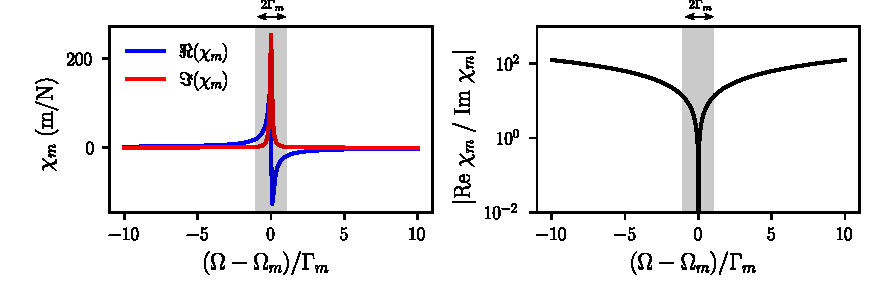
\includegraphics[width=\textwidth]{./chap3/fig/chi_meca.pdf}
  \caption{DYes}
  \label{fig:freq_indep_squeezing}
\end{figure}

\noindent \textbf{Convergence to VIRGO/LIGO notation:} We once again show that this general treatment converges to the one used in the context of gravitational wave detectors. In the free mass regime, $\mathcal{K}[\Omega]$ is real, such that $\phi_m[\Omega]=0$. One can then rewrite the optimal squeezing angle as
\begin{equation}
  \theta[\Omega] = \arctan \Big[\dfrac{2\mathcal{K}[\Omega]}{1 + \mathcal{K}^2[\Omega]}\Big] = \arctan \mathcal{K}[\Omega]
\end{equation}
where we used the identity $\arctan 2x/(1+x^2) = 2\arctan x \, \, (\text{mod}\, \pi)$, such that this comes down to the expression used in the context of gravitational wave detectors \cite{harry_advanced_2010, aasi_enhanced_2013}.


\subsection{Filter Cavities for Frequency Dependent Squeezing}

To generate frequency dependent squeezed states, one can use a filter cavity to rotate the squeezing angle in a frequency dependent manner. The filter cavity is a detuned optical cavity, such that such that symmetrical sidebands around the carrier will experience different phase shifts upon reflection. 

Recalling the transfer matrix for a detuned single port cavity from the previous chapter 
\begin{equation}
\mathbf{T}_{\mathrm{r}}[\Omega] = \mathbf{\Gamma} \, \mathbf{r}_{\Delta}[\Omega] \, \mathbf{\Gamma}^{-1} = \frac{1}{2}  \begin{pmatrix}
    r_{\Delta}[\Omega] + r_{\Delta}^*[-\Omega] & i(r_{\Delta}[\Omega] - r_{\Delta}^*[-\Omega]) \\
    -i(r_{\Delta}[\Omega] - r_{\Delta}^*[-\Omega]) & r_{\Delta}[\Omega] + r_{\Delta}^*[-\Omega]
  \end{pmatrix}
\end{equation}




\section{Cavity Optomechanics with Membrane based systems }
\subsection{Classical Description}
To gain intuition and derive elementary parameters used in the next section, we first describe the classical fields $\alpha_L$ and $\alpha_R$ propagating in a three mirror cavity where a membrane with complex amplitude reflection and transmission coefficients \(r_m=|r_m|e^{i\phi_r}\) and \(t_m=|t_m|e^{i\phi_t}\) is placed between two high reflectivity mirrors of amplitude reflection coefficients \( \sim -1 \). The membrane splits the cavity in two sub-cavities of lengths \(L_1\) and \(L_2\), with \(L=L_1+L_2\) the total cavity length. The membrane is initially at mean position $x=0$, and is modelled as a thin dielectric slab of thickness \(d\) and refractive index \(n\), with amplitude reflection and transmission coefficients \(r_m\) and \(t_m\) given by \cite{thompson_strong_2008}
\begin{equation}
r_m = \frac{(n^2-1)\sin k n d}{2 i n \cos k n d  + (n^2+1)\sin k n d}, \qquad t_m = \frac{2 n}{2 i n \cos k n d  + (n^2+1)\sin k n d}. 
\end{equation}
In the lossless case, we will assume the index of refraction $n$ is real, such that \(|r_m|^2 + |t_m|^2 = 1\). The cavity fields are then written as
\begin{equation}
\begin{split}
\alpha_R &= t_m \alpha_L + r_m \alpha_R' \\ 
\alpha_L' &= t_m \alpha_R' + r_m \alpha_L. \\
\end{split}
\end{equation}
In this case, energy conservation i.e. $|\alpha_L|^2 + |\alpha_R'|^2 = |\alpha_L'|^2 + |\alpha_R|^2$ imposes that $2(\phi_t-\phi_r) = \pi$ such that we can chose $r_m = |r_m|$ and $t_m = i|t_m|$. We rewrite the the cavity fields by injecting the identities $\alpha_L = - \alpha_L' e^{2ikL_1}$ and $\alpha_R' = - \alpha_R e^{2ikL_2}$ i.e. end mirror reflectivities of -1, leading to
\begin{equation}
   (t_m^2 - r_m^2) e^{ikL} - e^{-ikL}  = 2 r_m \cos(2kL_2 - kL )
\end{equation}
leading to the transcendental equation \cite{jayich_dispersive_2008}
\begin{equation}
  -\cos kL = |r_m|\cos (2kL_2 - kL)
\end{equation}
Following the method in Sankey et al. \cite{sankey_strong_2010}, we then derive the cavity resonance frequencies as a function of the membrane position \(x\) around its mean position \(x=0\). We will also always consider a long cavity such that \( L \gg \lambda,x \). Consequently, the small displacement \(x\) of the membrane around its mean position will weakly affect the cavity resonance frequencies such that 
\begin{equation}
  k(x)x = \dfrac{\omega(x)}{c} x = \dfrac{N\omega_{FSR}}{c}x + \dfrac{\delta\omega}{c}x  \implies k_N x + \pi 
\end{equation}


The cavity sublenghts considering a non zero mean membrane position are then \(L_1 \rightarrow L_1 +  x\) and \(L_2 \rightarrow L_2 -  x\). The above equation then becomes
\begin{equation}
  -\cos kL = |r_m|\cos (2k(L_2 - L_1) - 2kx ) 
\end{equation}
We now consider cases : the historical Membrane In the Middle (MIM) model where $L_1 \sim L_2 \sim L/2$, and the less studied Membrane At The Edge (MATE) model where $L_1 \sim L \gg L_2$. By considering that the membrane displacement perturbs the cavity resonance frequency by an amount at most of the order of one FSR, expanding the the cosine on both sides with the standard trigonometric identities leads to     
\begin{equation}
  \begin{split}
    \text{MIM:} \quad \omega_c(x) & \simeq N \omega_{FSR} + \frac{c}{L} \arccos( (-1)^{N+1}|r_m| \cos 2 k  x) \\
    \text{MATE:} \quad \omega_c(x) & \simeq N \omega_{FSR} + \frac{c}{L} \arctan \Bigg( -  \dfrac{1 + |r_m|\cos 2 k  x}{|r_m|\sin 2kx} \Bigg)
  \end{split}
\end{equation}

\subsection{Quantum Langevin Equations}

Using the same tools as in section II.2, we can derive the QLE of a membrane based optomechanical system. The transmissive membrane splits the cavity in two sub-cavities of lengths \(L_1\) and \(L_2\), with \(L=L_1+L_2\) the total cavity length. The membrane position operator is described by annihilation operator $\hat x \propto \hat c + \hat c^{\dagger} $ as in the previous section. The central difference with the standard book-keeping optomechanical system of a mirror on a spring is that the membrane splits the cavity in two sub-cavities, such that two bosonic operators \(\hat a_L\) and \(\hat a_R\) are required to describe the intracavity fields. The membrane position then modifies the resonance frequencies of the two subcavities, such that they both depend on the membrane position as \(\omega_L(x)\) and \(\omega_R(x)\) but with inverse trend: when one cavity shortens and its FSR increases, the other lengthens and its FSR decreases. To first order, we can linearize the resonance frequencies as
\begin{equation}
\omega_L(\hat x) \simeq \omega_{L,0} + G_L \hat x, \qquad \omega_R(x) \simeq \omega_{R,0} + G_R \hat x,
\end{equation}
with \(G_L = \omega_{L,0}/L_1\) and \(G_R = - \omega_{R,0}/L_2\) the optomechanical couplings of the two subcavities, and where \(\omega_{L,0}\) and \(\omega_{R,0}\) are the unperturbed resonance frequencies of the two subcavities. 
The system now features a network of optical modes varying linearly with the membrane position, coupled by the membrane transmission. The Hamiltonian of this system can then be written as 
\begin{equation}
  \begin{split}
    \hat{H} = & \,  \hbar \, \omega_{L,0} \, \hat a_L^\dagger \hat{a}^{\vphantom{\dagger}}_L + \hbar \, \omega_{R,0} \, \hat{a}_R^\dagger \hat{a}_R^{\vphantom{\dagger}} + + \hbar \, \Omega_m \hat c^\dagger \hat c \\
    & + \hbar \,  (G_L \,  \hat a_L^\dagger \hat{a}_L^{\vphantom{\dagger}} + G_R \, \hat a_R^\dagger \hat{a}_R^{\vphantom{\dagger}}) \,  \hat x  \\
    & - \hbar \, J(\hat{a}_L^\dagger \hat{a}_R^{\vphantom{\dagger}} + \hat{a}_R^\dagger \hat{a}_L^{\vphantom{\dagger}})  
  \end{split}
\end{equation}
where we only considered one cavity mode per subcavity, and where \(J\) is the photon tunneling rate through the membrane, proportional to the membrane transmission \(t_m\). The first line describes the free evolution of the two subcavity modes and the mechanical resonator, the second line describes the optomechanical interaction between the membrane position and the two subcavity modes, while the third line describes the photon tunneling through the membrane.


\subsubsection{Classical Description : Closed cavity model}
We start by describing the classical behaviour of the cavity. Considering a high finesse cavity, with high reflectivity mirrors \(r_1, r_2 \approx 1\), the cavity fields are written as 
\begin{equation}
\begin{aligned}
\alpha_1 = \alpha_1'
\end{aligned}
\end{equation}
where \(E_{\mathrm{in}}\) is the input field, \(E_1\) the intracavity field before the membrane, \(E_2\) the intracavity field after the membrane, \(E_3\) the transmitted field and \(E_4\) the reflected field. The cavity resonance frequencies are then obtained by solving these equations in the absence of input field \(E_{\mathrm{in}}=0\), leading to the transcendental equation \cite{jayich_dispersive_2008}



We describe the subcavity modes by annihilation operators \( \hat a_1\) and \(\hat a_2\), with unperturbed resonance frequencies \(\omega_1\) and \(\omega_2\). The membrane position operator is described by annihilation operator $\hat x \propto \hat c + \hat c^{\dagger} $ as in the previous section. Considering how the membrane position under the effect of radiation pressure modifies the resonance frequencies of the two subcavities, the subcavity length can be written as \(L_1 = L_{1,0} +  x\) and \(L_2 = L_{2,0} -  x\), with \(L_{1,0}\) and \(L_{2,0}\) the equilibrium lengths, and $x$ the mean static displacement of the membrane. This mean displacement being small compared to the cavity length, we can linearize the resonance frequencies as
\begin{equation}
\omega_1(x) \simeq \omega_{0} + G_1 x, \qquad \omega_2(x) \simeq \omega_{0} - G_2 x,
\end{equation}
with \(G_1 = \omega_{0}/L_{1,0}\) and \(G_2 = \omega_{0}/L_{2,0}\) the optomechanical couplings of the two subcavities, and where \(\omega_{0}\) is the common frequency of the two modes i.e. \(\omega_{1,0} = \omega_{2,0} = \omega_{0}\). The system now features a network of optical modes varying linearly with the membrane position, coupled by the membrane transmission. The Hamiltonian of the system is then given by \cite{xu_cavity_2016}
\begin{equation}
\hat{H} = \hbar \omega_1(x) \hat a_1^\dagger \hat{a}_1 + \hbar \omega_2(x) \hat{a}_2^\dagger \hat{a}_2 + \hbar g(\hat{a}_1^\dagger \hat{a}_2 + \hat{a}_2^\dagger \hat{a}_1) + \frac{\hat{p}^2}{2m} + \frac{1}{2} m \omega_m^2 \hat{x}^2
\end{equation}


Two configurations are then possible: position the membrane at approximately half the total cavity length \(L/2\), such that \(L_{1,0} \simeq L_{2,0}\) and \(G_1 \simeq G_2\); or position the membrane close to one of the mirrors, such that one subcavity is much shorter than the other, e.g. \(L_{1,0} \gg L_{2,0}\) and \(G_1 \ll G_2\). The first configuration is called the \emph{membrane-in-the-middle} (MIM) configuration, while the second one is called the \emph{membrane-at-the-edge} (MATE) configuration. The MIM configuration has been widely studied in the literature \cite{jayich_dispersive_2008, thompson_strong_2008, sankey_strong_2010, xu_cavity_2016}, and has been used to demonstrate various quantum effects such as ponderomotive squeezing \cite{purdy_observation_2013}, quantum non-demolition measurements of phonon number \cite{sankey_strong_2010}, or ground-state cooling of a mechanical resonator \cite{peterson_laser_2016}. However, the MIM configuration suffers from a low optomechanical coupling rate due to the small value of \(G_{1,2}\), which limits its use for quantum experiments. The MATE configuration has been less studied, but offers a much larger optomechanical coupling rate due to the large value of \(G_1\). This makes it a promising candidate for quantum experiments. In this work, we will focus on the MATE configuration.












































\subsubsection*{Set-up and notation}
We consider a three–mode optical model for a membrane-at-the-edge (MATE) cavity with a \emph{highly transmissive} middle membrane. The long cavity mode is denoted by \(a\); the short cavity contributes two nearby modes, \(b_{+}\) and \(b_{-}\), centered \(\pm \lambda/4\) away in displacement. In the mode basis \((a,b_+,b_-)^\top\) we take (with \(\hbar=1\))
\begin{equation}
\label{eq:H}
\mathbf H=
\begin{pmatrix}
\delta_a & J & -J\\[2pt]
J & \delta_+ & 0\\[2pt]
-\,J & 0 & \delta_-
\end{pmatrix},
\qquad
\begin{aligned}
&\delta_a = r_m G_1\,\Delta x,\\
&\delta_\pm = r_m G_2\!\left(\Delta x \mp \frac{\lambda}{4}\right),
\end{aligned}
\end{equation}
with
\begin{equation}
J=\frac{c\,t_m}{2\sqrt{L_1L_2}},\qquad
t_m^2+r_m^2=1,\qquad
G_1=\frac{\omega_0}{L_1},\qquad
G_2=-\frac{\omega_0}{L_2}.
\end{equation}
Here \(\Delta x\) is the membrane displacement from the symmetry point, \(\lambda\) the optical wavelength, \(t_m\) (\(r_m\)) the middle-membrane amplitude transmission (reflection), and \(L_{1,2}\) the long/short sub-cavity lengths. High transmissivity means \(r_m\ll 1\) while \(J=O(t_m)\) can be sizable.

The exact normal modes are eigenoperators \(A_k=\alpha_k a+\beta_k b_+ + \gamma_k b_-\) obtained from \((\mathbf H-\omega_k\mathbb I)\,(\alpha_k,\beta_k,\gamma_k)^\top=0\). From the lower rows one finds the exact amplitude ratios
\begin{equation}
\label{eq:ratios}
\frac{\beta_k}{\alpha_k}=-\frac{J}{\delta_+-\omega_k},
\qquad
\frac{\gamma_k}{\alpha_k}=+\frac{J}{\delta_--\omega_k}.
\end{equation}
The ``physical'' orange branch in the figures is the one continuously connected to the long-cavity mode \(a\).

\section*{Time-domain adiabatic elimination}
Away from the two avoided crossings at \(\Delta x\approx\pm \lambda/4\), the short-cavity detunings \(|\delta_\pm-\omega|\) are large compared to the coupling:
\begin{equation}
\varepsilon_\pm \equiv \frac{J}{|\delta_\pm-\omega|}\ll 1 .
\end{equation}
The Heisenberg equations generated by \eqref{eq:H} read
\begin{equation}
\label{eq:EOM}
\begin{aligned}
i\dot a &= \delta_a a + J b_+ - J b_-,\\
i\dot b_+ &= \delta_+ b_+ + J a,\\
i\dot b_- &= \delta_- b_- - J a.
\end{aligned}
\end{equation}
The fast spectators \(b_\pm\) can be slaved to the slow variable \(a\) by setting \(\dot b_\pm\simeq 0\) to leading order:
\begin{equation}
\label{eq:slaving}
b_+ \simeq -\frac{J}{\delta_+}\,a,\qquad
b_- \simeq \phantom{-}\frac{J}{\delta_-}\,a.
\end{equation}
Substituting \eqref{eq:slaving} into the \(a\) equation in \eqref{eq:EOM} gives an effective single-mode dynamics
\begin{equation}
\label{eq:ae-effective}
i\dot a = \Bigg[\delta_a - J^2\!\left(\frac{1}{\delta_+}+\frac{1}{\delta_-}\right)\Bigg] a .
\end{equation}
Equation \eqref{eq:ae-effective} shows that, in the dispersive region, the spectators do not acquire population to leading order; they merely induce a frequency (phase) shift of the \(a\) mode of order \(J^2/\delta_\pm\).

If optical losses are included as \(\kappa_a,\kappa_\pm\) (phenomenologically via \(\delta_a\to\delta_a-i\kappa_a/2\) etc.), the same elimination yields
\begin{equation}
\label{eq:ae-loss}
i\dot a = \left[\delta_a-\frac{i\kappa_a}{2} - J^2
\left(\frac{1}{\delta_+ - i\kappa_+/2}+\frac{1}{\delta_- - i\kappa_-/2}\right)\right] a,
\end{equation}
and the validity condition strengthens to \(J\ll \sqrt{\Delta_\pm^2+\kappa_\pm^2/4}\) with \(\Delta_\pm=\Re(\delta_\pm-\omega)\).

\paragraph{Connection to eigenvectors.}
Using \eqref{eq:ratios}, for the branch connected to \(a\) one has \(|\beta/\alpha|,|\gamma/\alpha|=O(\varepsilon_\pm)\ll1\). Thus the \(b_\pm\) weights in the physical eigenoperator are \(O(\varepsilon_\pm^2)\), fully consistent with the slaving picture \eqref{eq:slaving}.

\subsubsection*{Closed form for the physical eigenfrequency}
The exact eigenvalue equation for the orange branch obtained from the first row of \((\mathbf H-\omega\mathbb I)v=0\) together with \eqref{eq:ratios} is
\begin{equation}
\label{eq:selfconsistent}
\omega \;=\; \delta_a - J^2\!\left(\frac{1}{\delta_+ - \omega}+\frac{1}{\delta_- - \omega}\right).
\end{equation}
In the dispersive regime \(|\delta_\pm|\gg |\omega|\) one can set \(\omega\to 0\) in the denominators at first order, giving the explicit approximation
\begin{equation}
\label{eq:omega-phys-first}
\boxed{\;
\omega_{\rm phys}(\Delta x)\;\approx\; r_m G_1\,\Delta x
- J^2\!\left[\frac{1}{r_m G_2(\Delta x-\tfrac{\lambda}{4})}
+\frac{1}{r_m G_2(\Delta x+\tfrac{\lambda}{4})}\right].
\;}
\end{equation}
Combining the two fractions yields a compact dispersive form
\begin{equation}
\label{eq:omega-phys-compact}
\boxed{\;
\omega_{\rm phys}(\Delta x)\;\approx\;
r_m G_1\,\Delta x
-\frac{2J^2}{r_m G_2}\,
\frac{\Delta x}{\Delta x^2-(\lambda/4)^2}\;.
\;}
\end{equation}
Close to the symmetry point \(|\Delta x|\ll \lambda/4\), \eqref{eq:omega-phys-compact} becomes nearly linear:
\begin{equation}
\label{eq:omega-linear}
\boxed{\;
\omega_{\rm phys}(\Delta x)\;\approx\;
\underbrace{\left[r_m G_1+\frac{32J^2}{r_m G_2\,\lambda^2}\right]}_{\text{renormalized slope}}
\,\Delta x .
\;}
\end{equation}
In the usual MATE limit \(L_1\gg L_2\) (hence \(|G_1|\ll |G_2|\)), the second term typically dominates the slope; this analytic form explains the gentle ``tilt'' of the orange branch between the two avoided crossings.

\subsubsection*{Schrieffer--Wolff (block-diagonal) derivation}
For completeness, write \(H=H_0+V\) with
\(
H_0=\mathrm{diag}(\delta_a,\delta_+,\delta_-)
\)
and
\(
V=\begin{psmallmatrix}
0 & J & -J\\ J & 0 & 0\\ -J & 0 & 0
\end{psmallmatrix}.
\)
Let \(S\) be anti-Hermitian satisfying \([H_0,S]=-V\).
A suitable choice is
\begin{equation}
S = 
\begin{pmatrix}
0 & \frac{J}{\delta_a-\delta_+} & -\frac{J}{\delta_a-\delta_-}\\[2pt]
-\frac{J}{\delta_a-\delta_+} & 0 & 0\\[2pt]
\frac{J}{\delta_a-\delta_-} & 0 & 0
\end{pmatrix}.
\end{equation}
The transformed Hamiltonian \(\tilde H=e^{S}He^{-S}=H_0+\frac{1}{2}[S,V]+O(J^3/\Delta^2)\) is block-diagonal to second order, with the \(a\) block
\begin{equation}
\label{eq:SW-effective}
H_{\rm eff}^{(a)}=\delta_a
- J^2\left(\frac{1}{\delta_+-\delta_a}+\frac{1}{\delta_--\delta_a}\right),
\end{equation}
which reduces to \eqref{eq:omega-phys-first} when \(|\delta_\pm|\gg |\delta_a|\). Residual \(a\!\leftrightarrow\!b_\pm\) couplings are suppressed to \(O(J^3/\Delta^2)\).

\subsubsection*{Local avoided crossings (breakdown of elimination)}
Near \(\Delta x\simeq +\lambda/4\), only \(b_+\) is near resonant; the relevant subspace is \((a,b_+)\) with
\begin{equation}
H_{\rm loc}^{(+)}=
\begin{pmatrix}
\delta_a & J\\ J & \delta_+
\end{pmatrix},
\qquad
\Rightarrow\qquad
\omega_{\pm}^{(+)}=\frac{\delta_a+\delta_+}{2}\pm
\sqrt{\left(\frac{\delta_a-\delta_+}{2}\right)^2+J^2}.
\end{equation}
The orange branch is the one connecting continuously to \eqref{eq:omega-phys-compact} away from the crossing. The same holds at \(\Delta x\simeq -\lambda/4\) with \(b_-\).
Adiabatic elimination is invalid in windows where \(\varepsilon_\pm\not\ll1\).

\section*{Validity conditions and practical rule}
The small parameter governing all steps is
\(
\varepsilon_\pm = J/|\delta_\pm-\omega|
\).
With losses,
\(
\varepsilon_\pm=J/\sqrt{\Delta_\pm^2+\kappa_\pm^2/4}
\).
A conservative working criterion is
\begin{equation}
\boxed{\;
\max\{\varepsilon_+,\varepsilon_-\}\lesssim 0.2\!-\!0.3
\quad\Rightarrow\quad
\text{errors in }\omega_{\rm phys}\text{ are }O(\varepsilon^2),\
\text{and }|b_\pm|^2/|a|^2=O(\varepsilon^2).
\;}
\end{equation}

\subsubsection*{Optional bright/dark re-basis}
Defining \(b_s=(b_+-b_-)/\sqrt2\) and \(b_d=(b_++b_-)/\sqrt2\), one finds that \(a\) couples only to the \emph{bright} mode \(b_s\) with strength \(\sqrt2\,J\), while \(b_d\) is dark to first order. In this basis the cubic spectrum becomes a quadratic (for \(a,b_s\)) plus a spectator \(b_d\) whose frequency lies near \(r_m G_2\Delta x\) and mixes weakly via \(O(r_m G_2\lambda/2)\). This re-basis is often convenient for fitting and for visualizing how the orange branch acquires its dispersive tilt.

\paragraph{Summary.}
In a high-\(T\) middle-membrane MATE system, the short-cavity modes are far detuned for most \(\Delta x\). They can be adiabatically eliminated, yielding the explicit orange-branch dispersion
\eqref{eq:omega-phys-compact} (or \eqref{eq:omega-linear} near the center), with controlled accuracy quantified by \(\varepsilon_\pm\). Only in narrow windows around \(\Delta x=\pm\lambda/4\) is a \(2\times2\) avoided-crossing description required.

\subsection{Mechanical Resonators}{Mechanical Resonators}
\subsection{Noise spectra}
We will derive the Hamiltonian formalism of a three mirror cavity, and show how it can be used to describe the optomechanical coupling of a membrane in the cavity.
We now have to consider two optical modes coupled to one another through the membrane transmitivities. The Hamiltonian of the system can be written as:
\begin{equation}
\hat{H} = \hbar \omega_1 \hat{a}_1^\dagger \hat{a}_1 + \hbar \omega_2 \hat{a}_2^\dagger \hat{a}_2 + \hbar g(\hat{a}_1^\dagger \hat{a}_2 + \hat{a}_2^\dagger \hat{a}_1) + \frac{\hat{p}^2}{2m} + \frac{1}{2} m \omega_m^2 \hat{x}^2
\end{equation}
where $\hat{a}_1$ and $\hat{a}_2$ are the annihilation operators of the two optical modes, $\omega_1$ and $\omega_2$ their respective frequencies, $g$ the optomechanical coupling strength, $\hat{p}$ and $\hat{x}$ the momentum and position operators of the membrane, $m$ its mass and $\omega_m$ its mechanical frequency. The optomechanical coupling strength $g$ is defined as:
\begin{equation}
g = \frac{\omega_1}{L} \sqrt{\frac{\hbar}{2 m \omega_m}} \left( T_1 + T_2 \right)
\end{equation}
where $T_1$ and $T_2$ are the transmitivities of the two optical modes through the membrane. The Hamiltonian can be diagonalized by introducing the normal modes of the system, which are the eigenstates of the Hamiltonian. The normal modes can be expressed as:
\begin{equation}
\hat{b}_1 = \frac{1}{\sqrt{2}} \left( \hat{a}_1 + \hat{a}_2 \right), \quad \hat{b}_2 = \frac{1}{\sqrt{2}} \left( \hat{a}_1 - \hat{a}_2 \right)
\end{equation}
The normal modes $\hat{b}_1$ and $\hat{b}_2$ are the symmetric and antisymmetric modes of the system, respectively. The Hamiltonian can then be rewritten in terms of the normal modes as:
\begin{equation}
\hat{H} = \hbar \omega_1 \hat{b}_1
^\dagger \hat{b}_1 + \hbar \omega_2 \hat{b}_2^\dagger \hat{b}_2 + \hbar g(\hat{b}_1^\dagger \hat{b}_2 + \hat{b}_2^\dagger \hat{b}_1) + \frac{\hat{p}^2}{2m} + \frac{1}{2} m \omega_m^2 \hat{x}^2
\end{equation}


\paragraph{Diagonalisation of two non-degenerate, tunnel-coupled optical cavities.}
Let \(a_{1}\) and \(a_{2}\) (with the usual bosonic commutation relations) annihilate photons in the first and second cavity, whose bare resonance frequencies are \(\omega_{1}\neq\omega_{2}\).  Photon tunnelling at rate \(J>0\) through the semi-transparent middle mirror couples the two modes, giving the second-quantised Hamiltonian
\[
H
  =\hbar
    \begin{pmatrix}
      a_{1}^{\dagger} & a_{2}^{\dagger}
    \end{pmatrix}
    \underbrace{\begin{pmatrix}
      \omega_{1} & J\\
      J          & \omega_{2}
    \end{pmatrix}}_{\,\mathbf M}
    \begin{pmatrix}
      a_{1}\\ a_{2}
    \end{pmatrix}.
\]
Diagonalising the \(2\times2\) Hermitian matrix \(\mathbf M\) one finds the normal–mode (super-mode) eigenfrequencies
\begin{equation}
\label{eq:split}
\omega_{\pm}= \frac{\omega_{1}+\omega_{2}}{2}\;\pm\;
              \sqrt{J^{2}+\bigl(\tfrac{\omega_{1}-\omega_{2}}{2}\bigr)^{2}},
\end{equation}
and introduces a mixing angle \(\theta\) via
\[
\tan 2\theta \;=\;\frac{2J}{\,\omega_{2}-\omega_{1}\,}, 
\qquad 0<\theta<\pi/2.
\]
The corresponding canonical operators
\[
A_{+}= \cos\theta\,a_{1}+\sin\theta\,a_{2},
\qquad
A_{-}=-\sin\theta\,a_{1}+\cos\theta\,a_{2},
\]
obey \([A_{\mu},A_{\nu}^{\dagger}]=\delta_{\mu\nu}\) and bring the Hamiltonian to the diagonal form
\[
H=\hbar\omega_{+}\,A_{+}^{\dagger}A_{+}\;+\;\hbar\omega_{-}\,A_{-}^{\dagger}A_{-},
\]
revealing two independent harmonic oscillators whose frequency splitting \(\omega_{+}-\omega_{-}=2\sqrt{J^{2}+[(\omega_{1}-\omega_{2})/2]^{2}}\) interpolates smoothly between the strong-coupling limit (\(\omega_{1}\approx\omega_{2}\)) and the large-detuning regime where each cavity mode retains its individuality and the admixture of its neighbour is suppressed by the small parameter \(J/|\omega_{2}-\omega_{1}|\ll1\).


